\documentclass[10pt]{article}
\usepackage{amsmath,amsthm,amssymb,dsfont,graphicx,xspace,epsfig,xcolor}
\usepackage{tikz, tkz-graph, tkz-berge}
\usetikzlibrary{decorations.pathreplacing}
\usetikzlibrary{patterns}
\usetikzlibrary{patterns.meta}
\usepackage{color}

\begin{document}

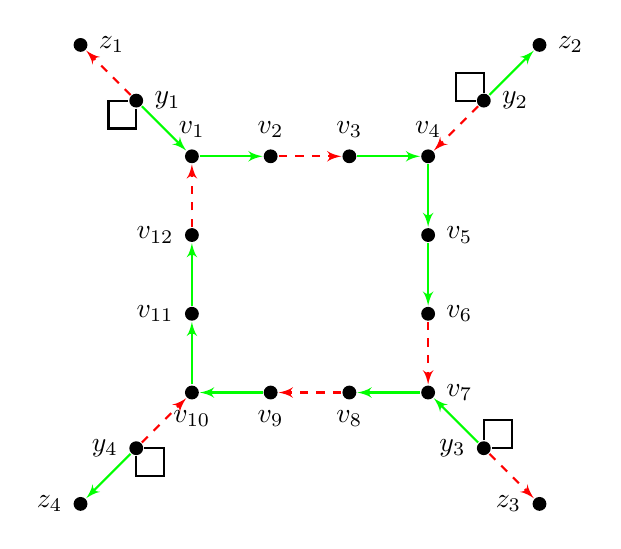
\begin{tikzpicture}[thick,scale=1, every node/.style={transform shape}]
    \tikzset{vertex/.style = {circle,fill=black,minimum size=5pt, inner sep=0pt}}
    \tikzset{edge/.style = {->,> = latex'}}
    \foreach \i in {0,...,3}{
        \pgfmathtruncatemacro{\j}{\i+1}
        \node[vertex, label=above:$v_\j$] (v\i) at (\i, 0) {};
    }
    \foreach \i in {1,2,3}{
        \pgfmathtruncatemacro{\j}{\i+4}
        \pgfmathtruncatemacro{\k}{\i+3}
        \node[vertex, label=right:$v_\j$] (v\k) at (3, -\i) {};
    }
    \foreach \i in {1,2,3}{
        \pgfmathtruncatemacro{\j}{\i+7}
        \pgfmathtruncatemacro{\k}{\i+6}
        \node[vertex, label=below:$v_{\j}$] (v\k) at (3-\i, -3) {};
    }
    \foreach \i in {1,2}{
        \pgfmathtruncatemacro{\j}{\i+10}
        \pgfmathtruncatemacro{\k}{\i+9}
        \node[vertex, label=left:$v_{\j}$] (v\k) at (0, -3+\i) {};
    }
    \foreach \i in {1,5,7,11}{
        \pgfmathtruncatemacro{\j}{Mod(\i+1,12)}
        \draw[edge, red, dashed] (v\i) to (v\j) {};
    }
    \foreach \i in {0,2,3,4,6,8,9,10}{
        \pgfmathtruncatemacro{\j}{Mod(\i+1,12)}
        \draw[edge,green] (v\i) to (v\j) {};
    }
    \node[vertex, label=right:$y_1$] (y1) at (-1/1.414,1/1.414) {};
    \node[vertex, label=right:$z_1$] (z1) at (-2/1.414,2/1.414) {};
    \draw[edge,green] (y1) to (v0) {};
    \draw[edge,red,dashed] (y1) to (z1) {};
    \draw (y1) -- (-1/1.414, 1/1.414 - 0.3535) -- (-1/1.414 - 0.3535, 1/1.414 - 0.3535) -- (-1/1.414 - 0.3535, 1/1.414) -- (y1);

    \node[vertex, label=right:$y_2$] (y2) at (3+1/1.414,1/1.414) {};
    \node[vertex, label=right:$z_2$] (z2) at (3+2/1.414,2/1.414) {};
    \draw[edge,red,dashed] (y2) to (v3) {};
    \draw[edge,green] (y2) to (z2) {};
    \draw (y2) -- (3+1/1.414, 1/1.414 + 0.3535) -- (3+1/1.414 - 0.3535, 1/1.414 + 0.3535) -- (3+1/1.414 - 0.3535, 1/1.414) -- (y2);

    \node[vertex, label=left:$y_3$] (y3) at (3+1/1.414,-3-1/1.414) {};
    \node[vertex, label=left:$z_3$] (z3) at (3+2/1.414,-3-2/1.414) {};
    \draw[edge,green] (y3) to (v6) {};
    \draw[edge,red,dashed] (y3) to (z3) {};
    \draw (y3) -- (3+1/1.414, -3-1/1.414 + 0.3535) -- (3+1/1.414+ 0.3535, -3-1/1.414 + 0.3535) -- (3+1/1.414+ 0.3535, -3-1/1.414) -- (y3);

    \node[vertex, label=left:$y_4$] (y4) at (-1/1.414,-3-1/1.414) {};
    \node[vertex, label=left:$z_4$] (z4) at (-2/1.414,-3-2/1.414) {};
    \draw[edge,red,dashed] (y4) to (v9) {};
    \draw[edge,green] (y4) to (z4) {};
    \draw (y4) -- (-1/1.414, -3-1/1.414 - 0.3535) -- (-1/1.414 + 0.3535, -3-1/1.414 - 0.3535) -- (-1/1.414 + 0.3535, -3-1/1.414) -- (y4);
\end{tikzpicture}

\end{document}